% ========================================================
\section{Résolution par la méthode des caracteristiques}
% ========================================================

\subsection{Méthode des caractéristiques}
L'équation du modèle \eqref{modele_McKendrick_Lotka} est une équation de transport, on peut donc la résoudre par la méthode des caracteristiques.
\\
Soit $a(X,t)$ la courbe caractéristique issue de $X \in \bbR$ fixé. La variation temporelle de $x$ le long de cette courbe s'écrit 
\begin{eqnarray*}
    \frac{\d}{\d t}x\big(a(X,t),t\big) = \frac{\partial a}{\partial t}
    (X,t)\frac{\partial x}{\partial a}\big(a(X,t),t\big)+\frac{\partial x}{\partial t}
    \big(a(X,t),t \big)
\end{eqnarray*}
En posant 
\begin{equation*}
    \frac{\partial a}{\partial t}(X,t) \equiv 1
\end{equation*}
on obtient 
\begin{eqnarray*}
    \frac{\d}{\d t}x\big(a(X,t),t\big) = 
    \frac{\partial x}{\partial a}\big(a(X,t),t\big)+\frac{\partial x}{\partial t}
    \big(a(X,t),t \big) = -\mu\big(a(X,t)\big)x\big(a(X,t),t\big)
\end{eqnarray*}
Déterminons $a$, on a 
\begin{eqnarray*}
    \frac{\partial a}{\partial t}(X,t) \equiv 1 
    &\Longrightarrow& a(X,t) = t + a(X,0)
\end{eqnarray*}
Si $X \geq 0$, on pose $a(X,0)=X$. Mais si $X<0$, on ne peut pas poser $a(X,0)=X$ car l'âge est positif, donc on pose $a(X,0)=0$. Cependant, pour $X<0$, la courbe caracteristique issue de $X$ ne démarre pas en $t=0$ mais en $t=-X$, donc on a aussi la condition 
\begin{equation*}
    a(X,-X) = 0
\end{equation*}
Finalement, pour tout $X \in \bbR$
\begin{eqnarray*}
    a(X,t) = t+X &\Longrightarrow& X = a-t
\end{eqnarray*}
et on a les conditions $t \in \bbR_+$ si $X \geq 0$ et $t \in [-X,+\infty[$ si $X<0$. 
\begin{figure}[!ht]
    \centering
    \begin{subfigure}{0.42\textwidth}
        \centering
        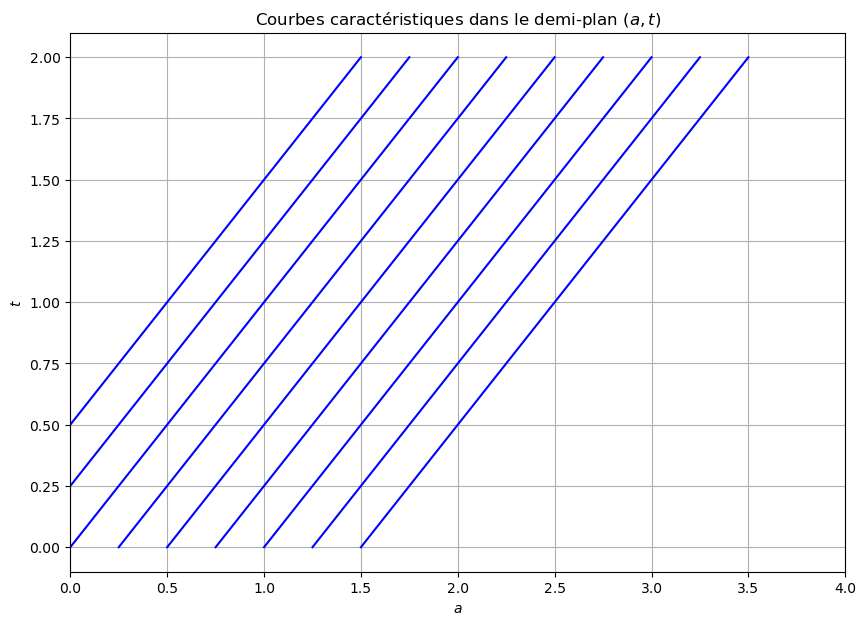
\includegraphics[width=\textwidth]{images/caracteristiques/caracteristiques1.png}
        \caption{Avec condition au bord}
    \end{subfigure}
    \hfill
    \begin{subfigure}{0.42\textwidth}
        \centering
        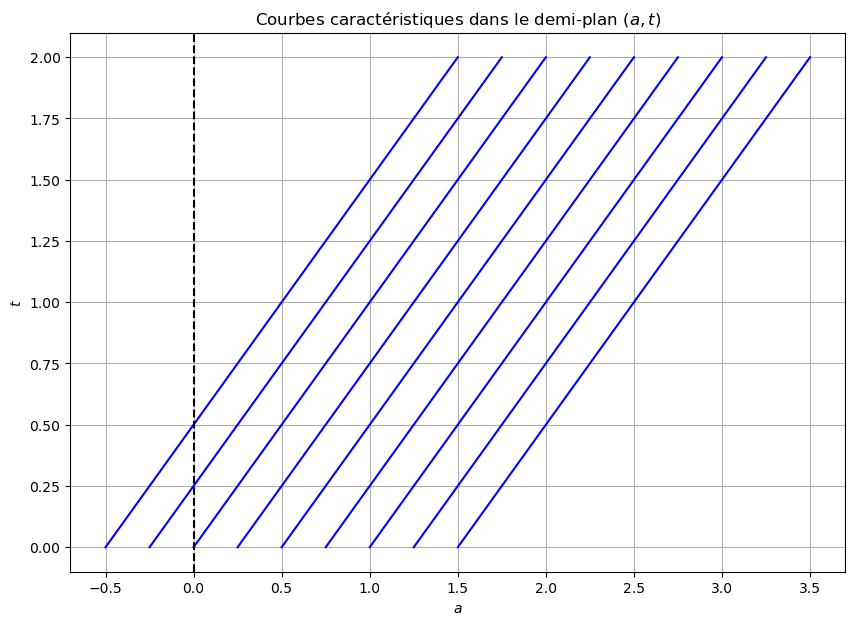
\includegraphics[width=\textwidth]{images/caracteristiques/caracteristiques2.png}
        \caption{Sans condition au bord}
    \end{subfigure}
    \caption{Caractéristiques dans le demi-plan $(a,t)$ avec et sans condition au bord}
    \label{fig:caracteristiques}
\end{figure}
\\

\begin{remark}
    Finalement, l'expression des caracteristiques est la même avec ou sans condition au bord. La seule différence est que, lorsqu'on a une condition au bord, on obtient une condition sur le temps $t$ et notre solution générale va être différente selon où se situe le pied de notre caracteristique.
\end{remark}

La solution générale est
\begin{equation*}
    x\big(a(X,t),t\big) = x\big(a(X,t_0),t_0\big)\exp\bigg(-\int_{t_0}^t\mu\big(a(X,s)\big)\d s\bigg)
\end{equation*}
où $t_0 \in \bbR$ est le temps de départ de la caracteristique.
\begin{itemize}
    \item Si $t_0=0$, on a $X \geq 0$ donc $a \geq t$. La solution
    est alors donnée par 
    \begin{eqnarray*}
        x(a,t) &=& x\big(a(X,0),0\big)\exp\bigg(-\int_{0}^t\mu\big(a(X,s)\big)\d s\bigg) \\
        &=& x_0(a-t)\exp\bigg(-\int_{0}^t\mu(a-t+s)\d s\bigg)
    \end{eqnarray*}
    \item Si $t_0=-X$, on a $X<0$ et donc $a<t$. La solution est 
    alors donnée par 
    \begin{eqnarray*}
        x(a,t) &=& x\big(a(X,-X),-X\big)\exp\bigg(-\int_{-X}^t\mu\big(a(X,s)\big)\d s\bigg) \\
        &=& x(0,t-a)\exp\bigg(-\int_{t-a}^t\mu(a-t+s)\d s\bigg) \\
        &=& B(t-a)\exp\bigg(-\int_{0}^a\mu(s)\d s\bigg)
    \end{eqnarray*}
\end{itemize}
La solution obtenue par la méthode des caractéristiques est donc 
\begin{eqnarray*}
    x(a,t) = \left\{\begin{array}{lc}
        x_0(a - t)\exp\bigg(-\displaystyle{\int_{0}^t}\mu (a-t+s)\d s\bigg) & \text{ si } a \geq t, \\
        & \\
        B(t-a)\exp\bigg(-\displaystyle{\int_0^a}\mu(s)\d s\bigg) & \text{ si } a < t.
    \end{array}\right.
\end{eqnarray*}
En utilisant les notations introduites précédemment, on peut réécrire 
\begin{equation}\label{sol_caracteristiques}
    x(a,t) = \left\{\begin{array}{lc}
        x_0(a - t)\dfrac{\Pi(a)}{\Pi(a-t)} & \text{ si } a \geq t, \\
        & \\
        B(t-a)\Pi(a) & \text{ si } a < t.
    \end{array}\right.
\end{equation}

\begin{remark}
    Il faut cependant rappeler que 
    \begin{equation*}
        B(t-a) = \int_0^{a_{\max}} \beta(\sigma)x(\sigma,t-a)\d \sigma
    \end{equation*}
    donc la solution $x$ donnée par \eqref{sol_caracteristiques}, dans le cas $a < t$, dépend d'elle même.
\end{remark}

\subsection{L'équation de renouvellement en démographie}
Dans cette section, on reprend les raisonnements de \cite{Iannelli2017, Brauer2019}.

\subsubsection{L'équation de renouvellement}
Maintenant qu'on a déterminé la solution, on peut réinjecter son expression dans la condition au bord. On obtient
\begin{eqnarray*}
    B(t) &=& \int_0^{a_{\max}} \beta(a)x(a,t)\d a \\
    &=& \int_0^t\beta(a)B(t-a)\Pi(a)\d a + \int_t^{a_{\max}} 
    \beta(a)x_0(a-t)\frac{\Pi(a)}{\Pi(a-t)}\d a \\
    &=& \int_0^t K(a)B(t-a)\d a + \underbrace{\int_0^{a_{\max}} \beta(a+t)x_0(a)\frac{\Pi(a+t)}{\Pi(a)}\d a}_{=:F(t)}
\end{eqnarray*}
où $K$ est la fonction de maternité définie précédemment. Pour le changement de variable, la borne supérieure était $a_{\max}-t$, on peut prendre $a_{\max}$. Et, on prolonge par $0$ les fonctions $\beta$, $\Pi$, et $x_0$ en dehors de $[0,a_{\max}]$. Finalement, on obtient \textcolor{astral}{\textit{l'équation de renouvellement}}
\begin{equation}\label{eq_renouvellement}
    B(t) = F(t)+\int_0^tK(a)B(t-a)\d a
\end{equation}

\begin{proposition}\label{thm_K_F}
    Avec les hypothèses faites précédemment sur $\beta$, $\mu$
    et $x_0$, on a 
    \begin{enumerate}
        \item $K \in L^{\infty}(\bbR_+)$ et pour presque tout $a \in \bbR_+$ on a 
        \begin{eqnarray*}
            \text{si } a \in [0,a_{\max}], \ 0 \leq K(a) \leq \beta_+
            \ \ \ &\text{ et }& \ \ \ \text{si } a > a_{\max}, \ K(a) = 0
        \end{eqnarray*}
        \item la fonction $F$ est continue sur $\bbR_+$ et 
        \begin{eqnarray*}
            \forall t \in [0,a_{\max}], \ 0 \leq F(t) \leq \beta_+\|x_0\|_{L^1}
            \ \ \ &\text{ et }& \ \ \ \forall t > a_{\max}, \ F(t) = 0
        \end{eqnarray*}
    \end{enumerate}
\end{proposition}

\begin{proof}
    \begin{enumerate}
        \item Comme on a prolongé par $0$ les fonctions $\beta$ et $\Pi$, on a également pour presque tout $a > a_{\max}$
        \begin{equation*}
            K(a) = 0
        \end{equation*}
        Comme les fonctions $\beta$ et $\Pi$ sont positives, $K$ aussi et on a 
        \begin{equation*}
            K(a) \leq \beta_+ \Pi(a) \leq \beta_+
        \end{equation*}
        donc $K \in L^{\infty}(\bbR_+)$.
        \item Si $t > a_{\max}$ alors $\beta(a+t) =0$ et donc 
        $F(t)=0$. De plus, on a 
        \begin{equation*}
            \beta(a+t) x_0(a)\frac{\Pi(a+t)}{\Pi(a)} \leq \beta_+x_0(a)
        \end{equation*}
        donc 
        \begin{equation*}
            F(t) \leq \beta_+ \|x_0\|_{L^1}
        \end{equation*}
        et $F$ est positive comme intégrale d'une fonction postive. Montrons que $F$ est continue. Soit $t_0 \in \bbR_+$.
        \begin{eqnarray*}
            |F(t)-F(t_0)| &=& \bigg|\int_0^{a_{\max}}\frac{x_0(a)}{\Pi(a)}\big(K(a+t)-K(a+t_0)\big)\d a \bigg| \\
            &\leq& \int_0^{a_{\max}} x_0(a)\beta_+|\Pi(a+t)-\Pi(a+t_0)|\d a 
        \end{eqnarray*}
        On a 
        \begin{equation*}
            x_0(a)\beta_+|\Pi(a+t)-\Pi(a+t_0)| \leq \beta_+x_0(a) 
        \end{equation*}
        et $\beta_+x_0 \in L^1(0,a_{\max})$ donc par le théorème de convergence dominée et par continuité de $\Pi$, on a 
        \begin{equation*}
            \lim_{t \to t_0} |F(t)-F(t_0)| = 0
        \end{equation*}
        donc $F$ est continue sur $\bbR_+$.
    \end{enumerate}
\end{proof}

\subsubsection{Résolution de l'équation de renouvellement}
Il nous faut à présent résoudre \eqref{eq_renouvellement}, c'est-à-dire déterminer $B \in \scrC^0(\bbR_+,\bbR)$ qui vérifie \eqref{eq_renouvellement}. La régularité $\scrC^0$ est justifiée par le fait que $F$ soit continue.

\begin{theorem}
    L'équation de renouvellement \eqref{eq_renouvellement} admet une unique solution continue $B$ qui satisfait 
    \begin{equation}\label{estim_renouv_B}
        \forall t \in \bbR_+, \ 0 \leq B(t) \leq \beta_+\ex^{\beta_+ t}\|x_0\|_{L^1}
    \end{equation}
\end{theorem}

\begin{proof}
    L'équation \eqref{eq_renouvellement} ressemble à un problème de point fixe. On va donc définir, pour $t \in \bbR_+$, la suite $(B_k(t))_{k \in \bbN}$ par récurrence comme 
    \begin{eqnarray}\label{eq_renouvellement_suite}
        B_0(t) &=& 0 \nonumber \\
        B_{k+1}(t) &=& F(t) + \int_0^tK(s)B_{k}(t-s)\d s
        = F(t) + \int_0^tK(t-s)B_{k}(s)\d s 
    \end{eqnarray}
    Montrons par récurrence que pour tout $k \in \bbN$, $t \mapsto B_k(t)$ est positive et continue sur $\bbR_+$.
    \begin{itemize}
        \item Initialisation : Il est clair que $B_0$ est positive et continue.
        \item Hérédité : Supposons que $B_k$ soit positive et continue. Montrons que $B_{k+1}$ est positive et continue. On sait que $F$ et $K$ sont positives, de plus, par hypothèse de récurrence $B_k$ est aussi positive. Donc $B_{k+1}$ est positive comme somme de deux fonctions positives. Enfin, pour montrer que $B_{k+1}$ est continue il suffit de montrer que $t \mapsto \displaystyle{\int_0^t} K(s)B_k(t-s)\d s$ est continue, car $F$ est continue par le théorème \ref{thm_K_F}. On utilise la majoration sur $K$ donnée par le théorème \ref{thm_K_F}
        \begin{eqnarray*}
            \bigg|\int_0^t K(s)B_k(t-s)\d s - \int_0^{t_0} K(s)B_k(t_0-s)\d s\bigg| &=& \bigg|\int_{\bbR_+} \big(K(s)B_k(t-s)\mathds{1}_{[0,t]}(s)\\
            &-& K(s)B_k(t_0-s)\mathds{1}_{[0,t_0]}(s)\big)\d s\bigg| \\
            &\leq& \beta_+ \int_{\bbR_+}\big|B_k(t-s)\mathds{1}_{[0,t]}(s)\\
            &-& B_k(t_0-s)\mathds{1}_{[0,t_0]}(s)\big|\d s
        \end{eqnarray*}
        On a bien par hypothèse de récurrence
        \begin{eqnarray*}
            \beta_+\big|B_k(t-s)\mathds{1}_{[0,t]}(s)
            - B_k(t_0-s)\mathds{1}_{[0,t_0]}(s)\big| &\underset{t \to t_0}{\longrightarrow}& 0
        \end{eqnarray*}
        et si on se restreint à un voisinage de $t_0$ (car on veut faire tendre $t$ vers $t_0$)
        \begin{equation*}
            \beta_+\big|B_k(t-s)\mathds{1}_{[0,t]}(s)
            - B_k(t_0-s)\mathds{1}_{[0,t_0]}(s)\big| \leq 2\beta_+\sup_{u \in [0,t_0+1]}|B_k(u)|\mathds{1}_{[0,t_0+1]}(s) \in L^1(\bbR_+)
        \end{equation*}
        donc par le théorème de convergence dominée
        \begin{eqnarray*}
            \bigg|\int_0^t K(s)B_k(t-s)\d s - \int_0^{t_0} K(s)B_k(t_0-s)\d s\bigg| &\underset{t \to t_0}{\longrightarrow}& 0
        \end{eqnarray*}
        d'où la continuité de $t \mapsto B_{k+1}(t)$ sur $\bbR_+$.
    \end{itemize}
    Soit maintenant $T >0$ et soit $t \in [0,T]$. On sait par le raisonnement précédent que $B_k \in \scrC^0([0,T])$ pour tout $k \in \bbN$. On a 
    \begin{eqnarray*}
        |B_{k+1}(t) - B_k(t)| &\leq& \int_0^tK(t-s)|B_k(s)-B_{k-1}(s)|\d s \\
        &\leq& \beta_+ \int_0^t |B_k(s)-B_{k-1}(s)|\d s
    \end{eqnarray*}
    En appliquant l'inégalité à nouveau on obtient 
    \begin{eqnarray*}
        |B_{k+1}(t) - B_k(t)| &\leq& \beta_+^k\|B_1-B_0\|_{L^{\infty}}\int_0^t \int_0^{s_1}\int_0^{s_2} \cdots \int_{0}^{s_{k-1}} \d s_k \cdots \d s_2 \d s_1 \\
        &=& \beta_+^k \frac{t^k}{k!}\|B_1-B_0\|_{L^{\infty}} \\
        &\leq& \beta_+^k \frac{T^k}{k!}\|B_1-B_0\|_{L^{\infty}}
    \end{eqnarray*}
    Ainsi,
    \begin{equation*}
        \sum_{k=1}^{+\infty}\|B_{k} - B_{k-1}\|_{L^{\infty}}\leq \|B_1-B_0\|_{L^{\infty}} \sum_{k=1}^{+\infty}\frac{(\beta_+ T)^k}{k!} = \|B_1-B_0\|_{L^{\infty}} \big(\ex^{\beta_+ T} - 1\big) < +\infty
    \end{equation*}
    donc la série de terme général $B_{k} - B_{k-1}$ est normalement convergente, donc convergente. Donc la suite des sommes partielles définie par 
    \begin{equation*}
        B_n = \sum_{k=1}^nB_{k}-B_{k-1}
    \end{equation*}
    converge uniformément sur $[0,T]$ vers une fonction $B$ continue. Ainsi, en passant à la limite quand $k$ tend vers $+\infty$ dans \eqref{eq_renouvellement_suite} on obtient une solution de \eqref{eq_renouvellement} sur $[0,T]$. A présent, il nous faut montrer l'unicité de la solution. Pour ça, on se donne une solution $\tilde{B}$ de \eqref{eq_renouvellement} sur $[0,T]$. Alors on a 
    \begin{equation*}
        |B(t)-\tilde{B}(t)| \leq \beta_+\int_0^t |B(s)-\tilde{B}(s)| \d s
    \end{equation*}
    On peut donc appliquer le lemme de Grönwall, on obtient
    \begin{equation*}
        \forall t \in [0,T], \ |B(t)-\tilde{B}(t)| \leq 0 \times \ex^{\beta_+t} = 0
    \end{equation*}
    donc pour tout $t \in [0,T]$, $B(t) = \tilde{B}(t)$. Et enfin, $T$ ayant été choisi quelconque dans $\bbR_+$, on a existence et unicité d'une solution $B \in \scrC^0(\bbR_+,\bbR)$.
\end{proof}

Maintenant qu'on a montré l'existence et l'unicité de $B$ pour \eqref{eq_renouvellement}, on peut revenir à l'équation \eqref{eq_McKendrick_Lotka}.

\begin{theorem}
    Si $B$ est solution de \eqref{eq_renouvellement} alors $x$ définie par \eqref{sol_caracteristiques} est l'unique solution de \eqref{modele_McKendrick_Lotka}. De plus, $x$ est continue sur $[0,a_{\max}] \times \bbR_+$ avec $a<t$. Enfin, pour $(a,t) \in [0,a_{\max}] \times \bbR_+$ on a $x(a,t) \geq 0$,
    \begin{equation*}
        x \in \scrC^0\big([0,T], L^1(0,a_{\max})\big)
    \end{equation*}
    et l'estimation
    \begin{equation*}
        \|x(t)\|_{L^1} \leq \ex^{\beta_+t}\|x_0\|_{L^1}
    \end{equation*}
\end{theorem}

\begin{proof}
    L'expression \eqref{sol_caracteristiques} vérifie clairement \eqref{modele_McKendrick_Lotka}. De plus, la continuité de $x$ pour $a<t$ sur $[0,a_{\max}] \times \bbR_+$ est évidente par continuité de $B$ sur $\bbR_+$ et de $\Pi$ sur $[0,a_{\max}]$. L'unicité de la solution $x$ est donnée par l'unicité de $B$. La positivité est également immédiate avec le théorème sur $B$. Enfin, on a l'estimation 
    \begin{eqnarray*}
        \forall t \in [0,T], \ \|x(t)\|_{L^1} &=& \int_0^t B(t-a)\Pi(a)\d a + \int_t^{+\infty} x_0(a-t)\frac{\Pi(a)}{\Pi(a-t)}\d a \\
        &=&\int_0^t B(t-a)\Pi(a)\d a + \int_0^{+\infty} x_0(a)\frac{\Pi(a+t)}{\Pi(a)}\d a \\
        &\leq& \bigg(\beta_+\int_0^t \ex^{\beta_+(t-a)}\d a+1\bigg)\|x_0\|_{L^1} \\
        &=& \ex^{\beta_+t}\|x_0\|_{L^1}
    \end{eqnarray*}
    donc $x \in \scrC^0\big([0,T], L^1(0,a_{\max})\big)$.
\end{proof}

\subsubsection{Comportement asymptotique}\label{sec_comportement_asymptotique_caracteristique}
Nous allons maintenant étudier le comportement asymptotique de $B$. Pour ça on va d'abord réécrire l'équation de renouvellement sous forme de convolution
\begin{equation*}
    B(t) = F(t) + (K*B)(t)
\end{equation*}
Puis on applique la transformée de Laplace à celle-ci, ce qui donne 
\begin{equation*}
    \hat{B}(z) = \hat{F}(z) + \hat{K}(z)\hat{B}(z)
\end{equation*}
où la transformée de Laplace est définie, pour une fonction $f : \bbR_+ \rightarrow \bbC$ localement intégrable sur $\bbR_+$, par 
\begin{equation*}
    \hat{f} : \bbC \rightarrow \bbC, \ z \mapsto \hat{f}(z)= \int_0^{+\infty} \ex^{-zs}f(s)\d s
\end{equation*}
Donc on a 
\begin{equation*}
    \hat{B}(z) = \frac{\hat{F}(z)}{1-\hat{K}(z)}
\end{equation*}
Par les propriétés de la transformée de Laplace, $\hat{K}$ et $\hat{F}$ sont analytiques donc les propriétés de $\hat{B}$ découlent du nombre de zéros de $1-\hat{K}$, autrement dit il nous faut résoudre l'équation suivante dans $\bbC$
\begin{equation}\label{eq_K_Laplace}
    \hat{K}(z) = 1
\end{equation}
On considère la fonction réelle
\begin{equation*}
    \hat{K}(x) = \int_0^{+\infty} \ex^{-xs}K(s)\d s
\end{equation*}
Par les propriétés de la transformée de Laplace, cette fonction est dérivable et on a par le théorème de dérivation sous le signe intégral
\begin{equation*}
    \forall x \in \bbR, \ \hat{K}'(x) = - \int_0^{+\infty}s\ex^{-xs}K(s)\d s < 0
\end{equation*}
donc $\hat{K}$ est strictement décroissante. On a aussi par le théorème de convergence dominée
\begin{eqnarray*}
    \lim_{x \to -\infty} \hat{K}(x) = +\infty \ \ \ &\text{ et }& \ \ \ \lim_{x \to +\infty} \hat{K}(x) = 0
\end{eqnarray*}
Par le théorème des valeurs intermédiraires, il existe un unique $\alpha^* \in \bbR$ tel que $\hat{K}(\alpha^*) = 1$. Il suit par stricte décroissance de $\hat{K}$ que 
\begin{eqnarray*}
    \alpha^* >0 &\iff& \hat{K}(\alpha^*) = 1 < \hat{K}(0) = R \\
    \alpha^* < 0 &\iff& \hat{K}(\alpha^*) = 1 > \hat{K}(0)=R
\end{eqnarray*}
Soit maintenant une autre solution $\alpha \in \bbC$ de \eqref{eq_K_Laplace} telle que $\alpha \neq \alpha^*$. Alors 
\begin{eqnarray*}
    \int_0^{+\infty} \ex^{-\alpha^*s}K(s)\d s &=& \Re\bigg(\int_0^{+\infty} \ex^{-\alpha s}K(s)\d s\bigg) \\
    &=& \int_0^{+\infty} \ex^{-\Re(\alpha) s}\cos{(\Im(\alpha)s)}K(s)\d s \\
    &\leq& \int_0^{+\infty} \ex^{-\Re(\alpha) s}K(s) \d s
\end{eqnarray*}
Si l'inégalité précédente est stricte alors $\Re(\alpha) < \alpha^*$. Et si on a égalité alors 
\begin{eqnarray*}
    \int_0^{+\infty} \ex^{-\Re(\alpha) s}\cos{(\Im(\alpha)s)}K(s)\d s &=& \int_0^{+\infty} \ex^{-\Re(\alpha) s}K(s) \d s \\
    &\Longrightarrow& \text{p.p.t. } \ s \in \bbR_+, \ \cos{(\Im(\alpha)s)}=1 \\
    &\Longrightarrow& \Im(\alpha) = 0
\end{eqnarray*}
donc $\alpha \in \bbR$ et par conséquent $\alpha = \alpha^*$, ce qui contredit l'hypothèse de départ. Donc toute solution de \eqref{eq_K_Laplace} admet une partie réelle strictement plus petite que $\alpha^*$.
\\
Par le théorème 5.2 de \cite{Iannelli1995}, on a 
\begin{equation*}
    B(t) = B_0\ex^{\alpha^*t}\big(1+\Omega(t)\big)
\end{equation*}
avec $B_0 \geq 0$ et $\displaystyle{\lim_{t \to +\infty}} \Omega(t)=0$. Donc avec \eqref{sol_caracteristiques}, on obtient 
\begin{equation*}
    \lim_{t \to +\infty} x(a,t) = \lim_{t \to +\infty} B_0\ex^{\alpha^*(t-a)}\Pi(a)
\end{equation*}
le signe de $\alpha^*$ va donc déterminer l'évolution de la population en temps long. Si $\alpha^*>0$ alors $R>1$ la population va croître de manière exponentielle. Si $\alpha^*<0$ alors $R<1$ et la population va décroître de manière exponentielle. Le $\alpha^*$ joue ici le même rôle que le paramètre de Malthus $\alpha$ définit dans la section \ref{sec_modele_Malthus}, et on retrouve un comportement similaire en temps long.